\documentclass[a4paper]{article}
\usepackage[margin=1in]{geometry}
\usepackage{graphicx}
\usepackage{hyperref}
\usepackage{amsmath}
\usepackage{booktabs}
\usepackage{subcaption}
\usepackage{tikz}
\usepackage{pgfplots}
\usepackage{indentfirst}
\usepackage{float}
\setlength{\parindent}{2em}

\title{\textbf{VE216 Lab 3 Report: Feedback Control}}
\author{
    \Large Zhanhui Zhou
    \normalsize 518370910159
}
\date{\today}

\begin{document}
    \maketitle

    \section{Background}

        \subsection{Closed-Loop Transfer Function}
        The block diagram is shown in Fig.1
        \begin{align*}
            G_{cl}(s) &= \frac{Y(s)}{X(s)} = \frac{C(s)P(s)}{1+C(s)P(s)H(s)} \\
            \frac{E(s)}{X(s)} &= \frac{1}{1+C(s)P(s)H(s)}
        \end{align*}
        \begin{figure}[H]
            \centering
            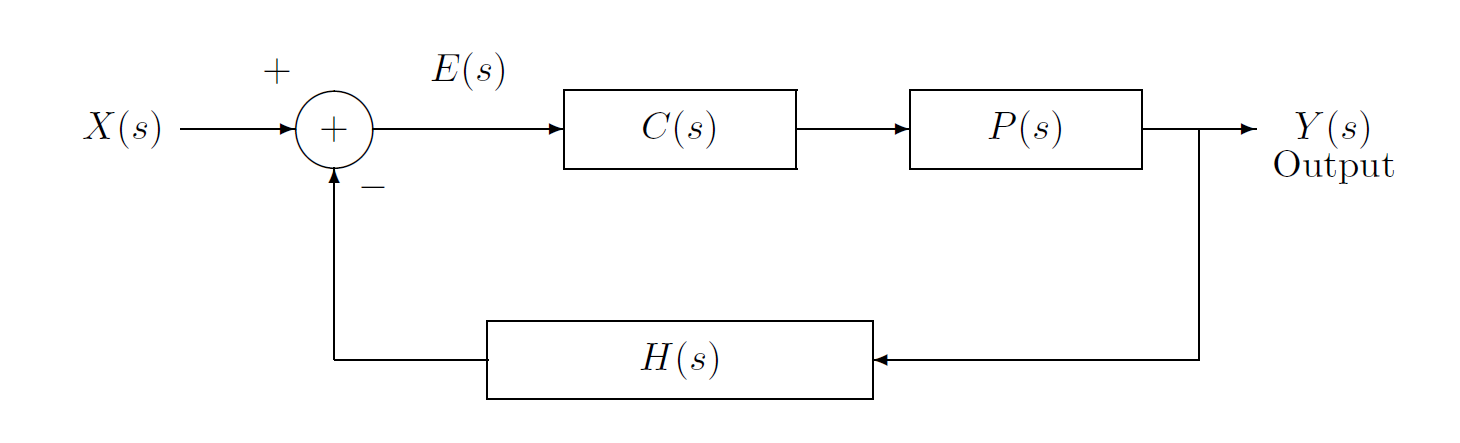
\includegraphics[width=12cm]{diagram.png}
            \caption{closed-loop feedback control system}
        \end{figure}

        \subsection{Examples of Feedback Control Systems}

            \subsubsection{DC Motor Model}
            The angular position, $\theta(t)$ is
            \begin{equation*}
                \frac{d^2\theta(t)}{dt^2} + \frac{d\theta t}{d(t)} = V(t)
            \end{equation*}
            with the system transfer function
            \begin{equation*}
                P(s) = \frac{1}{s(s+1)}
            \end{equation*}

            \subsubsection{No controller}
            If the input to the above function is a unit step. Then
            \begin{equation*}
                \theta(s) = V(s)P(s) = \frac{1}{s}\frac{1}{s(s+1)} = -\frac{1}{s} + \frac{1}{s^2} + \frac{1}{s+1}
            \end{equation*}
            Consequently, 
            \begin{equation*}
                \theta(t) = (t-1+e^{-t})u(t)
            \end{equation*}
            which is not going to achieve the desired rotation.

            \subsubsection{Controller Without Feedback}
            Shown in Fig.2 is the block diagram of an open-loop controller.
            \begin{figure}[H]
                \centering
                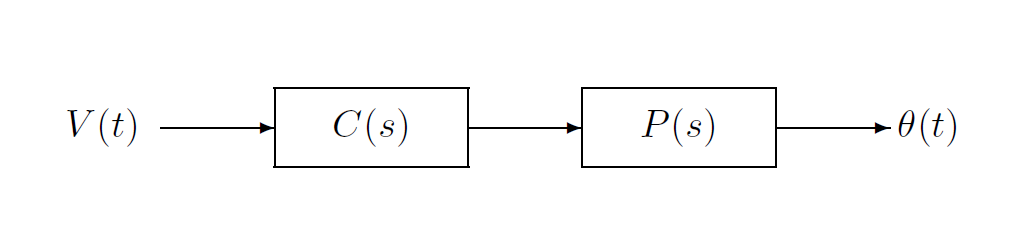
\includegraphics[width=12cm]{openloop.png}
                \caption{open-loop controller}
            \end{figure}

            With unit-step as input,
            \begin{equation*}
                \theta(s) = \frac{1}{s} - \frac{1}{s+1}
            \end{equation*}
            With ramp as input,
            \begin{equation*}
                \theta(s) = -\frac{1}{s} + \frac{1}{s^2} + \frac{1}{s+1}
            \end{equation*}


            \subsubsection{Feedback Control}
            Consider the system shown in \autoref{fig:closed_loop_diagram} with $H(s)=1$, $C(s)=Ks$ and $P(s) = 1/[s(s+1)]$. Then step response becomes
            \begin{equation*}
                \theta(s) = V(s)G_{cl}(s) = \frac{1}{s}\frac{K}{s+(K+1)} = \frac{K/(K+1)}{s} - \frac{K/(K+1)}{s+(K+1)}
            \end{equation*}
            or equivalently, 
            \begin{equation*}
                \theta(t) = \frac{K}{K+1}(1-e^{-(K+1)t})u(t)
            \end{equation*}

            \subsubsection{Sensitivity of an Open-Loop Controller to Plant Changes}
            It can be shown that the open-loop controller is sensitive to variations in the plant transfer function.

            \subsubsection{Using Feedback to Stabilize Unstable Systems}
            It can be shown that feedback system can stablize unstable systems.


    \section{Experiment Procedures}
    \subsection{Open Loop Control: Plant}

    \begin{itemize}
        \item Construct the plant with $R_0 = 10k\Omega, \, C_1 = 100\mu F, \, C_2 = 0.22\mu F$.
        \item Impulse response: A = 1V, width = 0.1s, f = 1Hz.
        \item Step response: A = 1V, f = 1Hz
    \end{itemize} 
        \subsection{Feedback Control}

        \begin{itemize}
            \item Add the feedback contorl circuit to the plant with $R_1 = R_3 = 150k\omega, \, R_2 = 3k\omega, \, C_3 = 0.47\mu F$
            \item Impulse response: A = 1V, width = 0.1s, f = 1Hz.
            \item Step response: A = 1V, f = 1Hz.
        \end{itemize}


    \section{Experiment Result}
    \paragraph{Open Loop Control - Plant}
    The experiment result for input and output of open loop control plant circuit is shown as followed.

    \begin{figure}[H]
        \centering
        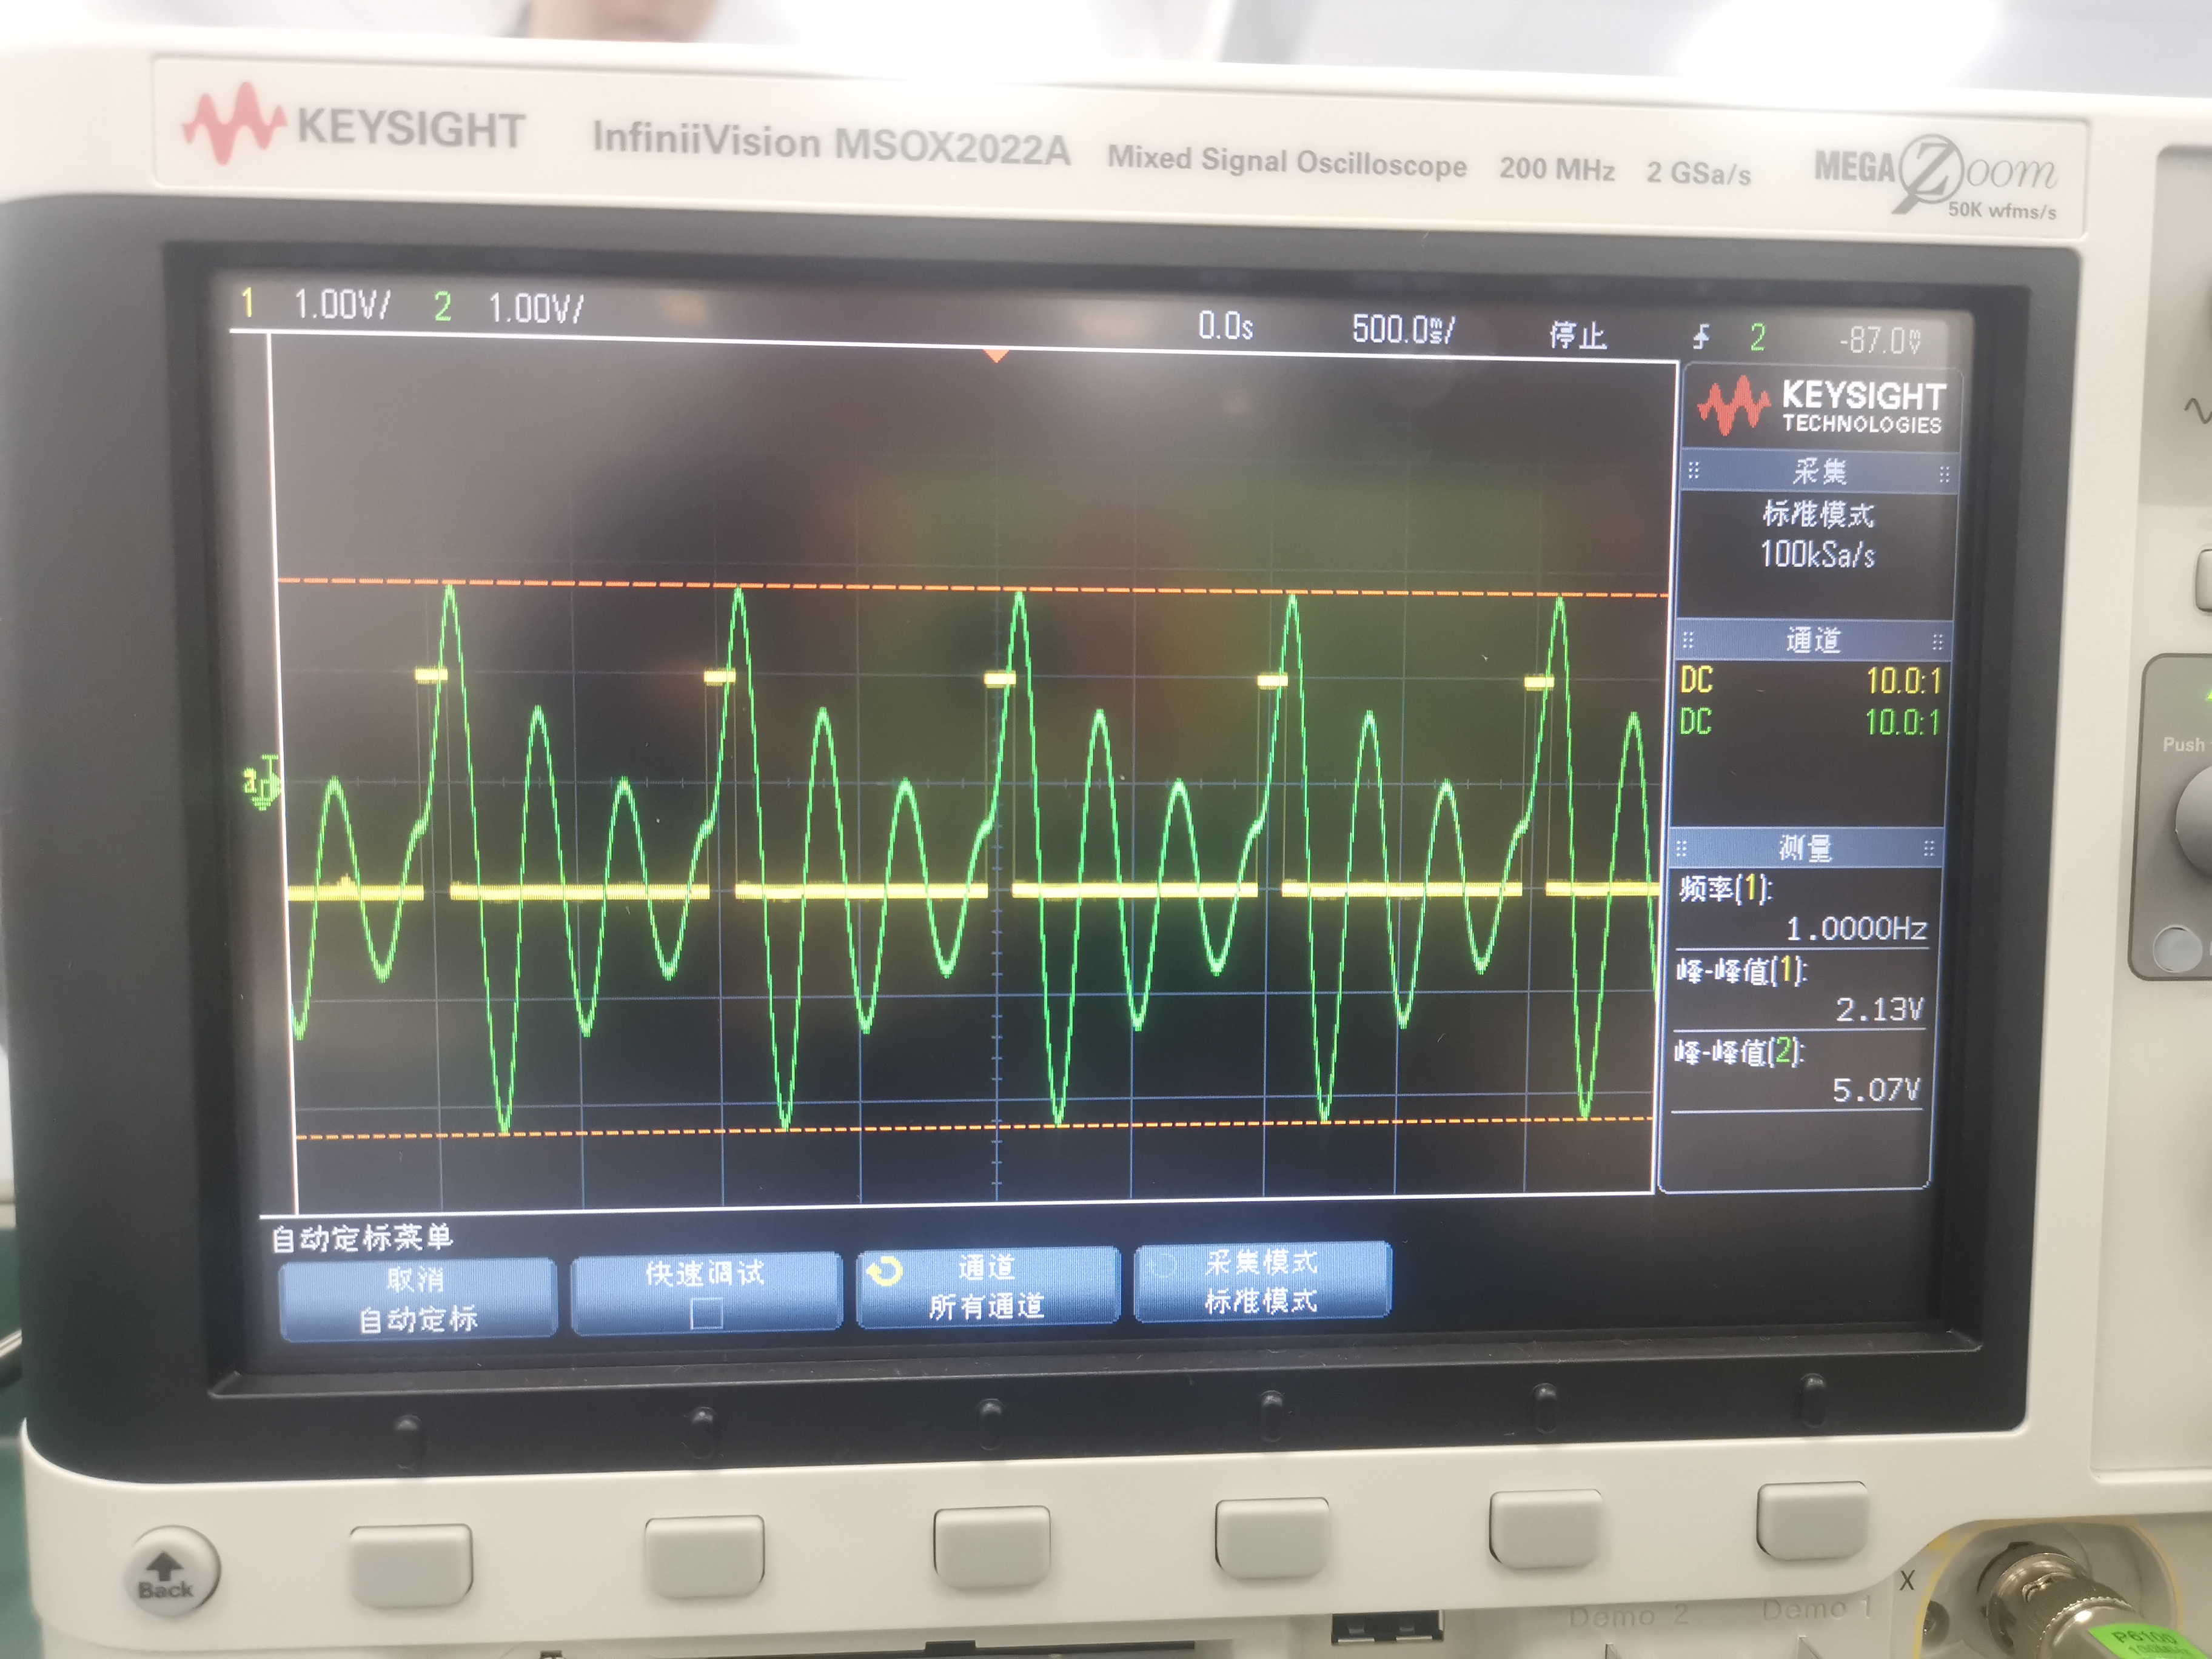
\includegraphics[width=10cm]{pulse1.jpg}
        \caption{Result of open loop control plant circuit of impulse}
    \end{figure}

    \begin{figure}[H]
        \centering
        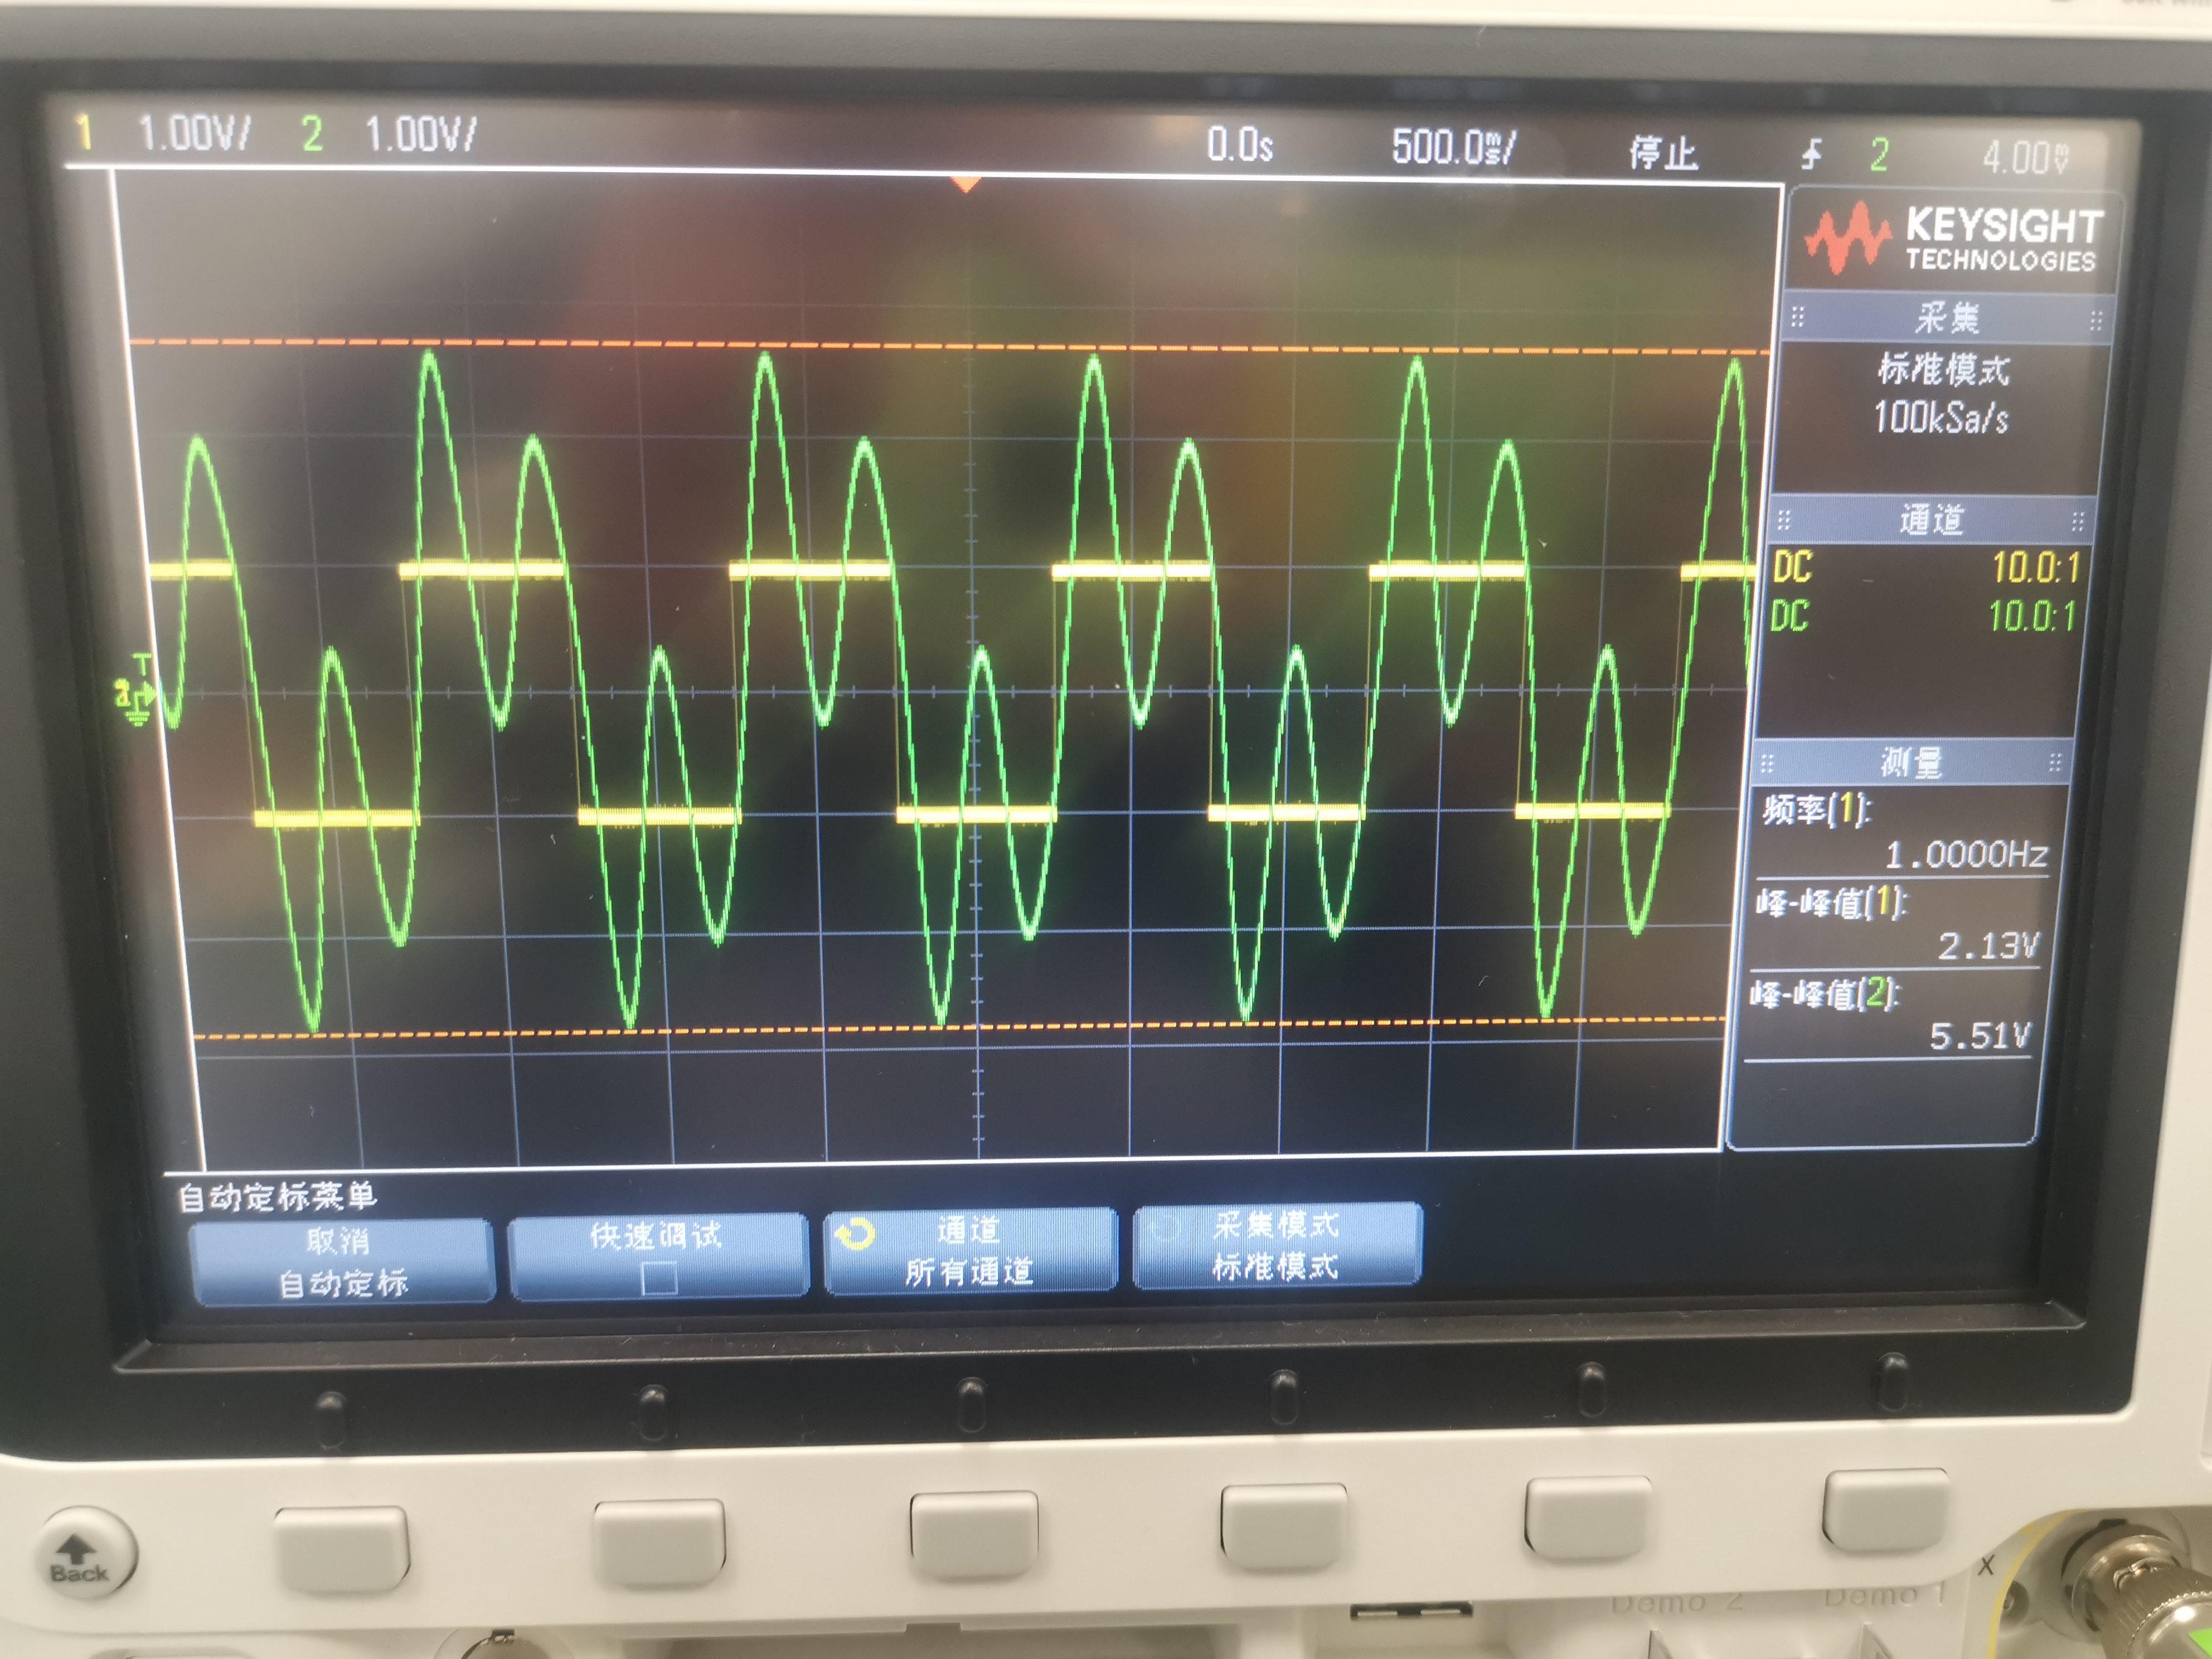
\includegraphics[width=10cm]{rect1.jpg}
        \caption{Result of open loop control plant circuit of step}
    \end{figure}

    \paragraph{Open Loop Control - Plant}
    The experiment result for input and output of feedback control circuit is shown in followed

    \begin{figure}[H]
        \centering
        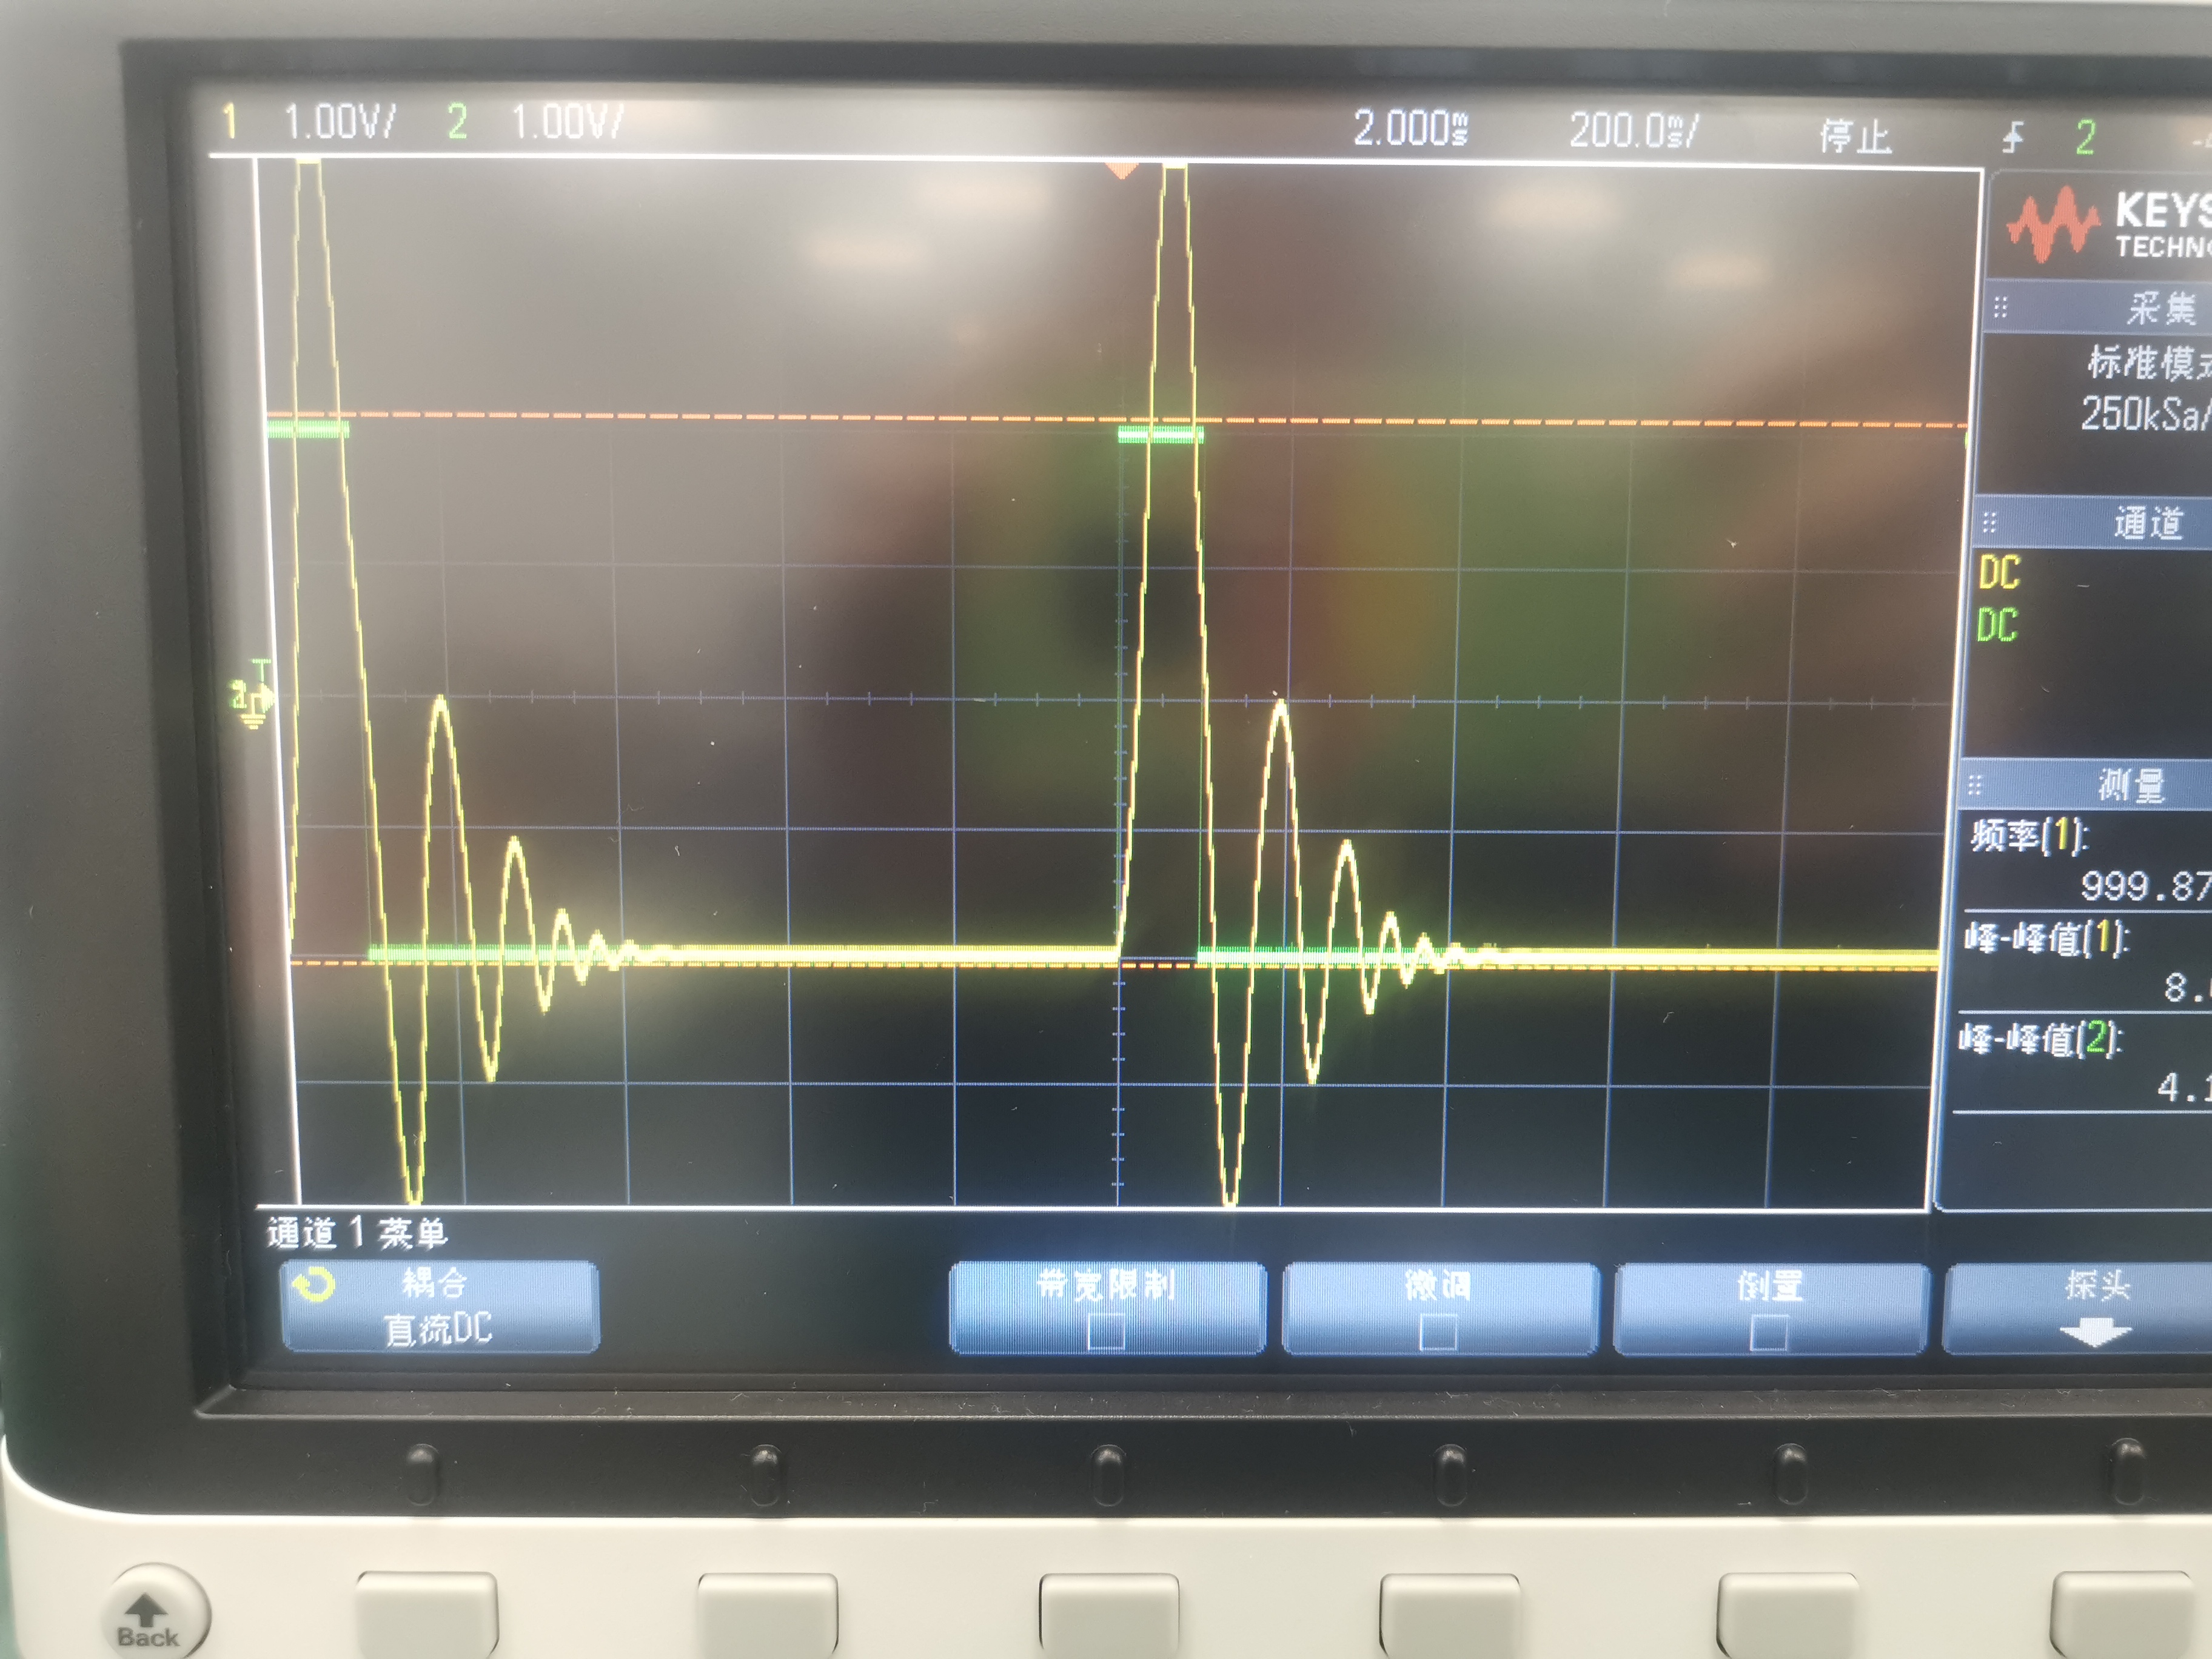
\includegraphics[width=10cm]{impulse2.jpg}
        \caption{Result of feedback control circuit of impulse}
    \end{figure}

    \begin{figure}[H]
        \centering
        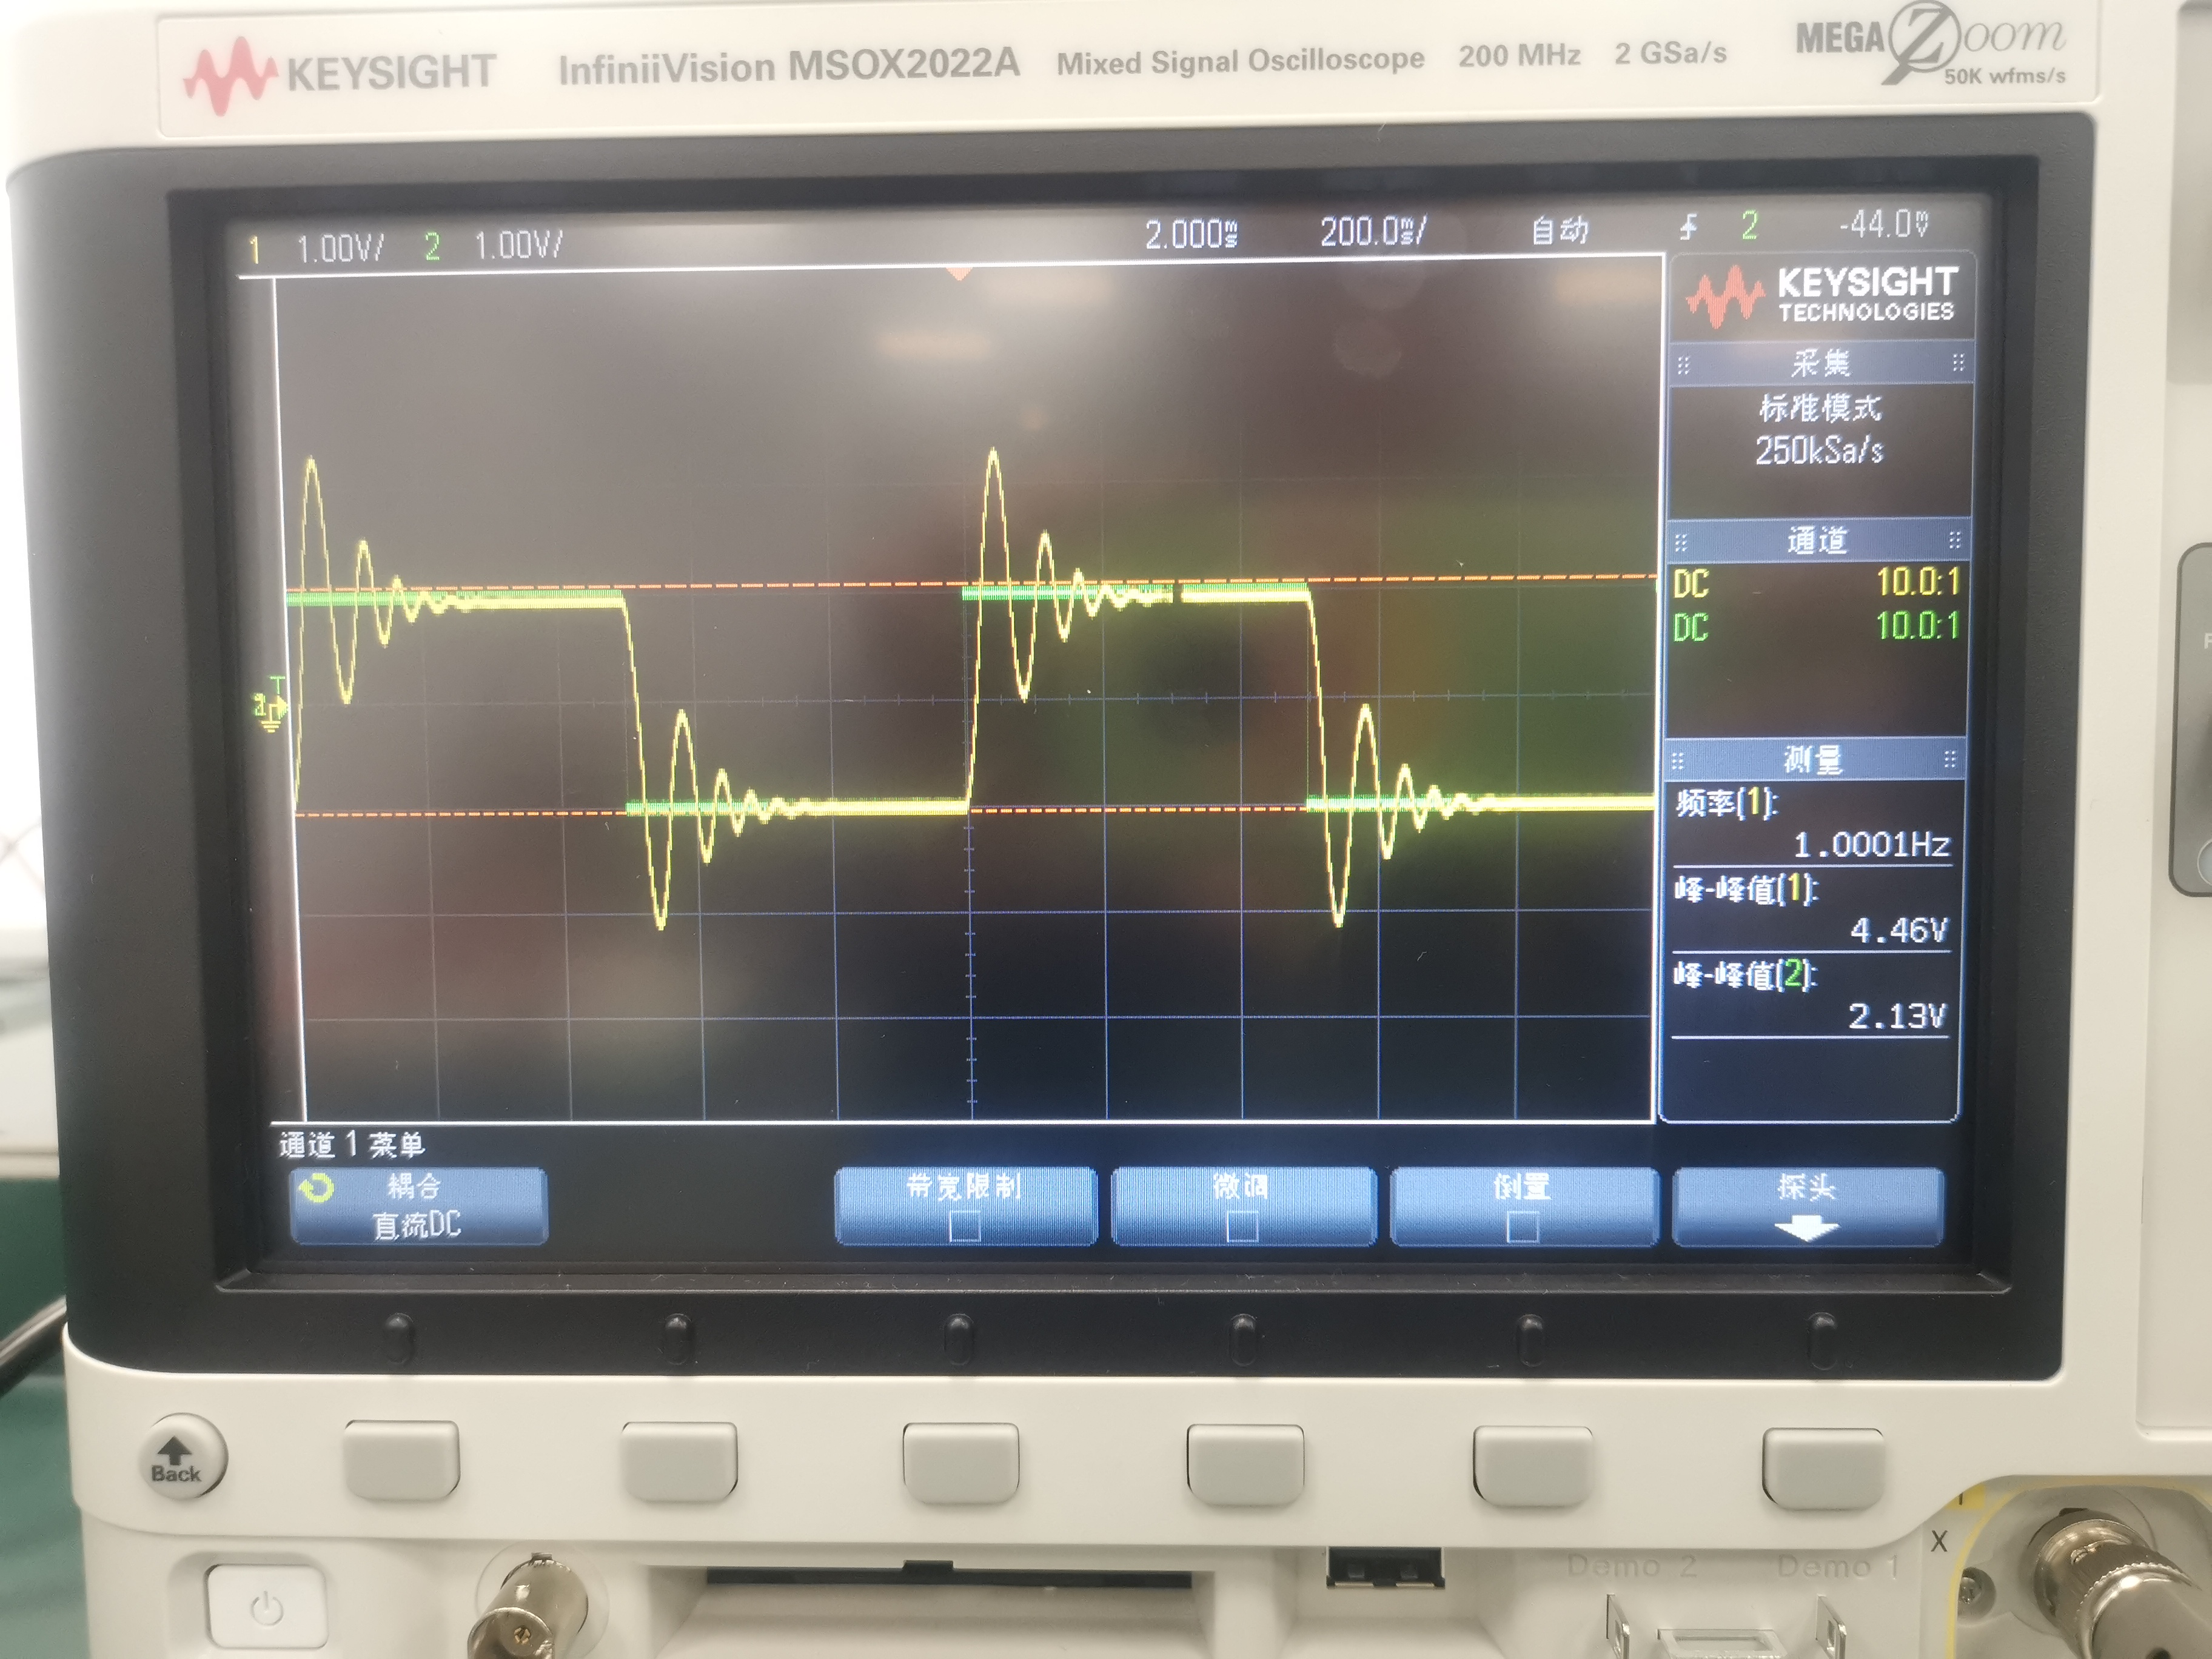
\includegraphics[width=10cm]{step2.jpg}
        \caption{Result of feedback control circuit of step}
    \end{figure}


    \section{Discussion and Error Analysis}
    By comparing the output of the feedback circuit and the tested circuit, it can be found that the feedback circuit can better stabilize the unstable system. \par
    
    The experimental results are in good agreement with the experimental results.

    \section{Conclusion}
    In this lab, I knew how to set up a plant and feedback control system, and how feedback systems stabilize unstable systems.

\end{document}